\documentclass[12pt,letterpaper]{article}
\usepackage[utf8]{inputenc}
\usepackage{float}
\usepackage{pdflscape}
\usepackage{amsmath}
\usepackage{amsfonts}
\usepackage{amssymb}
\usepackage{fullpage}
\usepackage{gensymb, comment}
\usepackage{textcomp}
\usepackage{threeparttable}
\usepackage{graphicx}
\usepackage[sort]{natbib}
\usepackage{setspace} 
\doublespacing
\usepackage{indentfirst}
\setlength{\parindent}{25pt}
\usepackage{bbm}
\usepackage{multicol}
\usepackage{makecell}
\usepackage{booktabs}
\newtheorem{prop}{Proposition} 
\newtheorem{assumption}{Assumption} 
\newtheorem{implication}{Implication} 
\usepackage{longtable}

\setcounter{totalnumber}{8}

\title{Winter weather on exam dates and matriculation for a prestigious university in Japan}%: \\ Empirical analysis on auditing reports in Brazil}
%\author{Mizuhiro Suzuki\thanks{Department of Agricultural and Applied Economics, University of Wisconsin-Madison. Contact: msuzuki7@wisc.edu. The author would like to thank Laura Schechter for her numerous feedback and support. I am also grateful to Joshua Deutschmann, Paul Dower, Jeremy Foltz, Priya Mukherjee, Andrew Stevens, and seminar participants at the UW-Madison Agricultural and Applied Economics department for helpful comments and suggestions. Any errors in this draft are the sole responsibility of the author.}}
\author{
  Mizuhiro Suzuki\thanks{
    Department of Agricultural and Applied Economics, University of Wisconsin-Madison.
    Contact: msuzuki7@wisc.edu.
    The author would like to thank Laura Schechter for her numerous feedback and support.
    I am also grateful to Daiji Kawaguchi for helpful comments and suggestions.
    Any errors are the sole responsibility of the author.
  }
}
\date{\today \\ \vspace{1cm} Preliminary draft \\ Please do not cite or circulate}

\begin{document}
  
\maketitle
\begin{abstract}
  \singlespacing
    \noindent 
    Whereas there are growing numbers of studies on how heat affects cognitive performance at high-stakes settings, the effect of cold weather has been less studied.
    To fill this gap, I analyze the effects of winter weather on exam dates on performance at the centralized exam for university admission in Japan.
    Since students take the exam in their own prefectures, they are exposed to different weather conditions on the exam dates. 
    I find that low temperature and snow cumulated on the ground reduce matriculation shares for the most prestigious university in Japan, the University of Tokyo.
    This result suggests that the winter weather on exam dates worsens exam performance. 
    %The implications on how to design university admissions are discussed.

  \medskip
  \vspace{1cm}
  \noindent Keywords: Temperature, Education, University matriculation, Cognitive performance
\end{abstract}

\newpage

\section{Introduction}

University admission is an important step in life and can have consequences in later-life outcomes such as job occupation and earnings.\footnote{
  \citet{Hout2012} reviews the returns to college education in the context of the United States.
}
For admission selection, standardized exams have been widely used in many countries.\footnote{
  Examples include the Unites States, the United Kingdom, Brazil, China, South Korea, and Japan.
}
Given the importance, the results of the exams are expected to evaluate the exam takers' ability and knowledge correctly and are not supposed to be affected by seemingly irrelevant factors.
However, recent studies have shown that exam performance is sensitive to external factors.
One such factor is temperature:
heat on the exam days has been shown to affect exam results in high-stakes settings \citep{Park2020a, GraffZivin2020}.
What has been less studied in the literature is the impact of \textit{low} temperature.\footnote{
  One might think that, considering the on-going global \textit{warming}, the effect of low temperature is becoming less important.
  However, the future climate change can cause the sea-ice loss, which could result in the cold winters with severely low temperatures \citep{Kretschmer2016, Kim2014}.
  Hence, it is important to understand how low temperature can affect our economies and lives.
}

To fill this gap in the literature, this study analyzes the effect of winter weather on exam outcomes in Japan.
For admission, most public universities in Japan require high school seniors and graduates to take a centralized test, called National Center Test for University Admission (Center Test henceforth).
Students take the exam on the same dates in mid-January in their prefectures.\footnote{
  There are 47 prefectures in Japan.
}
This creates a variation in weathers to which they are exposed on the exam dates.

I use the weather on the dates of Center Test and investigate its effect on matriculation for the University of Tokyo (UTokyo henceforth).
UTokyo is a national university and known to be the most prestigious in Japan.\footnote{
  According to \citet{usnews}, UTokyo is the highest-ranked university in Japan (73rd ranked in the world ranking).
  The second highest-ranked university in Japan is Kyoto University, which is 125th ranked in the world ranking.
}
This allows me to attribute a reduction in matriculation shares to the worse exam performance, instead of the better performance which could induce students to choose better universities.

The econometric analyses show that low temperature and snow cumulated on the ground on exam dates reduce the matriculation share.
The estimates are not only statistically but also economically significant.
Changing the temperature on the exam dates from 3-6 $^o$C to below 0 $^o$C decreases the matriculation share by 0.18\%, which amounts to 9\% of the average or 22\% of the median matriculation shares.
The results provide implications for effective measures to be taken to mitigate the negative impact of winter weather.
These include preparing waiting rooms for exam takers to warm up for equalizing their pre-exam conditions or adjusting the importance of the scores at Center Test in the admissions process.

This study mainly contributes to the recent but growing literature of the effects of climate factors on the outcome of high-stakes exams.
Several previous studies have found the adverse effect of high temperature on learning, which exacerbates performance at exams \citep{Park2020b, Cho2017}.
More closely to my study, \citet{GraffZivin2020} and \citet{Park2020a} show that heat on exam dates decreases the scores at high-stakes exams in China and the U.S., respectively.
Considering the importance of the exam results for later life outcomes, it is important to understand how external factors such as temperature affect exam performance and what can be done to ameliorate such effects.
To complement the literature, I investigate the effect of \textit{low} temperature on exam performance.

This study also has a contribution to the literature on the economic impact of low temperature.
It has been shown with controlled experiments that cold stresses negatively affect such things as cognitive ability and memory, as reviewed in \citet{Taylor2016}.
However, evidence based on data in the field is scarce.
Country-level studies have shown a non-linear effect of temperature on economic growth, that is, both low and high temperature has a negative impact \citep{Burke2015}.
One study based on microdata is \citet{Stevens2017}, who finds a negative impact of low temperature on labor productivity of blueberry pickers in California.
I use prefecture-level information to investigate how low temperature affects the cognitive performance in a high-stakes exam.

This study proceeds as follows.
In Section \ref{sec:background}, the context of this study is introduced.
Section \ref{sec:data} describes the data. 
I introduce my empirical strategy in Section \ref{sec:empirical_strategy}.
In Section \ref{sec:results}, I present the empirical results, and Section \ref{sec:conclusion} concludes.
  
\section{Background}\label{sec:background}

In Japan, for admission to public universities, students are usually required to take two exams.
The first-stage test is Center Test.
Students take an exam on consecutive two days (Saturday and Sunday) in mid-January.
Most public universities, including UTokyo, require students to take exams on social science, Japanese, and English on the first day and mathematics and natural science on the second day.
The exams start at 9:30 AM on both days and end at 6:10 PM on the first day and 5:50 PM on the second day.
Questions are multiple-choice and common for all exam takers across Japan.
High-school seniors take the test at designated sites in the exam area\footnote{ \label{footnote:prefecture}
  Typically, an exam area coincides with a prefecture (i.e. there is one exam area in one prefecture).
  Large prefectures such as Hokkaido and Okinawa have several exam areas.
  Also, several municipalities in a prefecture can be sometimes considered to be a part of a neighboring prefecture.
  For instance, students in a couple of municipalities in Saitama prefecture could take Center Test in Tokyo.
} where their high schools are located.
On the other hand, high-school graduates are assigned to test sites in the exam area where the homes used in their applications are located.\footnote{
  \citet{Watanabe2013} provides detailed descriptions on the administrations of Center Test.
}

Since January is the middle of winter in Japan, heavy snow can affect public transportation on exam dates.
This sometimes makes it difficult for exam takers to arrive at exam sites on time.
For the affected students, the following accommodations can be provided:
(i) delaying the start of exams by a few hours for all exam takers at a test site,
(ii) allowing the affected students to take exams in a separate room, and
(iii) allowing the affected students to take make-up exams a week later.
These accommodations can be given to students who could not take exams for other reasons such as sickness or accidents.

After Center Test, applicants for public universities typically take the second-stage exam.
This exam is made by each university, and students physically go to the universities and take the exam.
Therefore, every applicant for a university takes the second-stage exam at the same location on the same days.
UTokyo has the second-stage exam at the end of February for two days.\footnote{
  Until 2015, UTokyo had another second-stage exam in March and a small number of exam takers got admitted through the exam (around 3\% of all admitted students).
  In 2016, UTokyo abolished the March exam and instead started to admit the small number of students recommended by their high schools based on interviews and scores at Center Test (around 2\% of all admitted students).
  Since the majority of students are admitted through the second-stage exam in February, below I focus on the admissions process for those students. 
}

In admission for UTokyo, scores at Center Test are used for two purposes.
First, the scores are used for eligibility to take the second-stage exam.
Thresholds varying across years and majors are set, and if scores at Center Test are below the thresholds, the students cannot take the second-stage exam.
Secondly, the scores at Center Test are taken into consideration for admission.
The final score of a student is calculated by the weighted sum of exam scores at the first- and second-stage exams.\footnote{
  In 2020, the weights for Center Test and the second-stage exam are 20\% and 80\%.
  Faculty of Medicine additionally conducts interviews on the next day of the second-stage exam to screen applicants based on community skills and personal maturity.
}

In summary, results at Center Test are crucial for applicants for UTokyo.
This study will investigate how external factors such as temperature and weather on the dates of Center Test affect matriculation for UTokyo.

\section{Data}\label{sec:data}

I use two sets of data: weather and matriculation for UTokyo.
For weather information, I obtain data from \Citeauthor{jma}.
Their website maintains the past weather across Japan.
Based on hourly weather on exam dates at prefecture capitals, I use average weather between 6 AM to 6 PM.
Prefecture capitals tend to be most populated in each prefecture, and highly-ranked high schools from which many students go to UTokyo are likely to be located at prefecture capitals.

For matriculation information for UTokyo, I use University Basic Information by \Citeauthor{univ_info}.
This data contains information from 2012 to 2020 on the number of matriculated students for each university by prefectures at which their high schools are located.
I calculate the matriculation shares of each prefecture as the ratio of the number of matriculated students from a prefecture to the number of all matriculated students.\footnote{
  Due to the lack of information on the number of admitted students by prefecture, I use the information on matriculation.
  For UTokyo, the number of admissions and the number of matriculations are very close:
  In 2020, among 3,083 admitted students, 3,064 students matriculated at UTokyo.
}

The summary statistics are provided in Table \ref{tab:sum_stat}.
Whereas the mean matriculation share is $2.08 \%$, the median share is much smaller ($0.79 \%$).\footnote{
  Since there are matriculations from foreign high schools, the mean value does not coincide with $1 / 47 \approx 2.12\%$.
  I do not consider matriculations of students from foreign high schools in the analyses since the majority of the students are admitted through a process called Special Screening Tests, which does not require Center Test scores.
}
This is because the distribution of the matriculation share is starkly skewed:
while the matriculation shares of the top 5 prefectures amount to more than 60\%, many prefectures have less than 1\% shares (Figure \ref{fig:admission_map}).


\begin{table}[H]
  \centering
  \caption{Summary Statistics}
  \resizebox{0.8\linewidth}{!}{
  
\begin{tabular}[t]{lllllll}
\toprule
\multicolumn{1}{c}{ } & \multicolumn{1}{c}{N} & \multicolumn{1}{c}{Mean} & \multicolumn{1}{c}{SD} & \multicolumn{1}{c}{Median} & \multicolumn{1}{c}{Min} & \multicolumn{1}{c}{Max} \\
\cmidrule(l{3pt}r{3pt}){2-2} \cmidrule(l{3pt}r{3pt}){3-3} \cmidrule(l{3pt}r{3pt}){4-4} \cmidrule(l{3pt}r{3pt}){5-5} \cmidrule(l{3pt}r{3pt}){6-6} \cmidrule(l{3pt}r{3pt}){7-7}
Matriculation share (\%) & 423 & 2.08 & 5.23 & 0.79 & 0.06 & 37.35\\
Temperature (\degree C) & 423 & 4.67 & 3.81 & 4.98 & -6.63 & 19.86\\
Hourly precipitation (mm) & 423 & 0.08 & 0.18 & 0.00 & 0.00 & 1.27\\
Hourly snowfall (m) & 423 & 0.00 & 0.00 & 0.00 & 0.00 & 0.01\\
Cumulated snow (m) & 423 & 0.05 & 0.15 & 0.00 & 0.00 & 1.26\\
\bottomrule
\end{tabular}

  }
  \label{tab:sum_stat}
  \footnotesize
  \begin{tablenotes}
    \item 
      Notes:
      Matriculation share (\%) is the share of newly matriculated students to the University of Tokyo from each prefecture.
      The matriculation share is calculated based on the ratio of the number of students from high schools in the prefecture to the total number of matriculation.
      I use weather variables at prefecture capitals between 6 AM and 6 PM on days of Center Test.
  \end{tablenotes}
\end{table}

\begin{figure}[H]
  \centering
  \caption{Map of matriculation shares (\%)}
  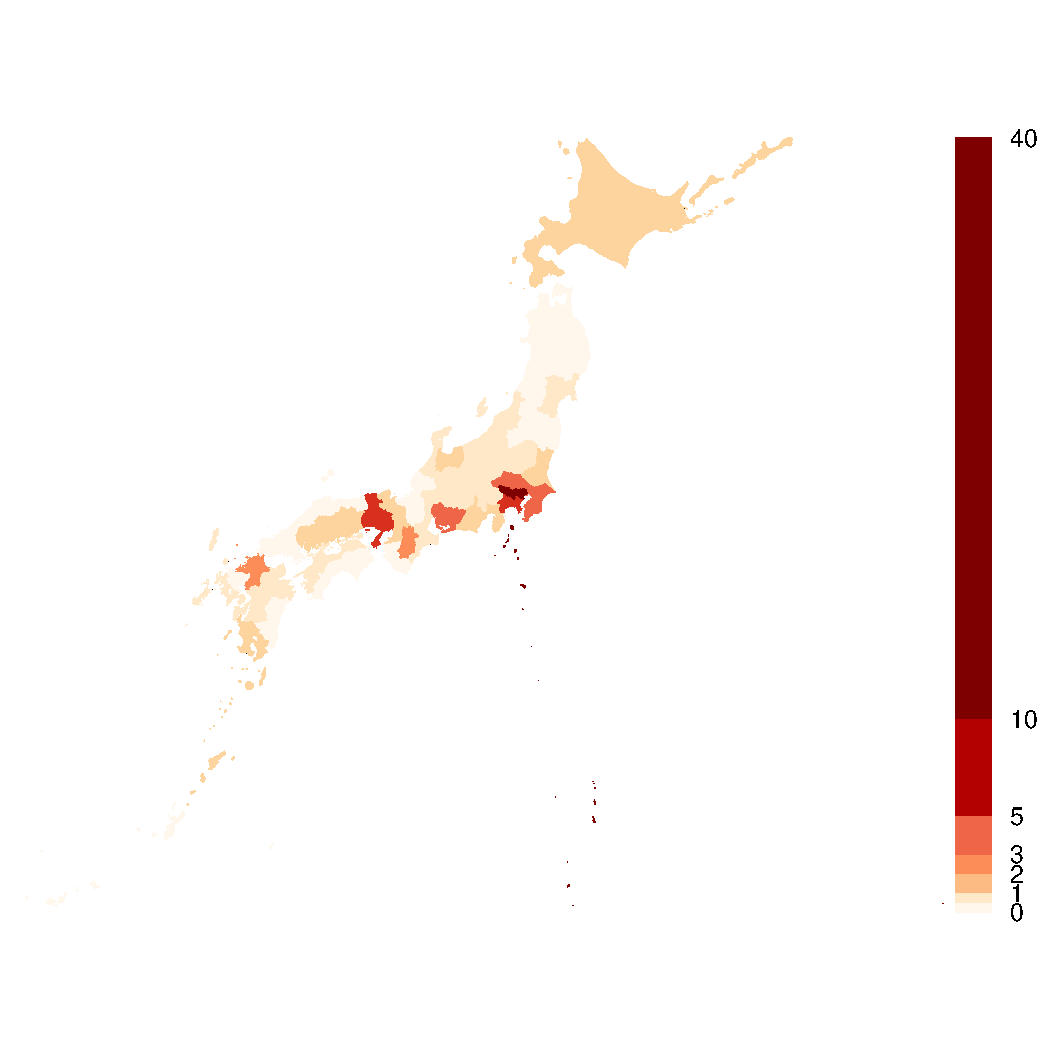
\includegraphics[width = 0.7\textwidth]{../Output/images/admission_map.pdf}
  \label{fig:admission_map}
  \footnotesize
  \begin{tablenotes}
    \item Notes:
      This map shows the matriculation shares (\%) for the University of Tokyo from each prefecture.
      The matriculation share is calculated based on the ratio of the number of students from high schools in the prefecture to the total number of matriculation.
      Average of the shares across years is shown in the map.
      Although not shown in the legend due to the lack of the space, the lightest color in the map means the matriculation share between 0 to 0.5\% 
  \end{tablenotes}
\end{figure}

\section{Empirical Strategy}\label{sec:empirical_strategy}

I analyze the effect of temperature and other weather variables on exam dates on the matriculation share for UTokyo.
The reason why I use the matriculation share for UTokyo is as follows:
consider a matriculation share for a middle-ranked university.
Suppose also that low temperature has a negative impact on exam scores.
Then, 
(i) students in the prefecture who would have gotten into the middle-ranked university if the temperature were higher may end up in a lower-ranked university instead, but
(ii) students in the prefecture who would have gotten into a higher-ranked university may end up in the middle-ranked university instead.
Hence, the matriculation share of the prefecture for the middle-ranked university may not be affected by low temperature.
However, the second effect is unlikely to be large for UTokyo since it is known to be the best university in Japan.\footnote{
  \citet{Kawaguchi2008} describes that ``The University of Tokyo has occupied the top position of the single-peaked university hierarchy since its establishment in 1877.''
}
Therefore, I rule out the second possibility and attribute a reduction in matriculation shares to the worse performance at Center Test.

In the analyses, the outcome variable, $Y_{jt}$, is the matriculation share (\%) for UTokyo of a prefecture $j$ in year $t$.
%Let $T_{jt}$ be the average temperature across two exam dates in $j$ in year $t$.
%I use functions of $T_{jt}$ in the regressions ($f$), which can be linear or non-linear.
The main right-hand side variable is temperature on the exam dates.
To allow for non-linear effects of temperature on the outcome, I use the 3-$^o$C temperature intervals.\footnote{
  The results with a linear specification are shown in Appendix \ref{sec:appendix_table} and will be discussed below.
}
Let $T_{jt}^k$ represent the $k$'th temperature bin.
I also include other weather variables such as rainfall, snowfall, and cumulated snow on the ground on exam dates as a vector $X_{jt}$.
As fixed effects, prefecture fixed effects ($\mu_j$) and year fixed effects ($\tau_t$) are used.
Finally, the error term is represented as $\epsilon_{jt}$.

Given the above notation, I run the following regression equation:
\begin{equation*}
  Y_{jt} = \sum_k T_{jt}^k + X_{jt}' \beta + \mu_j + \tau_t + \epsilon_{jt}.
\end{equation*}
I exploit the variation of temperature on exam dates, which I consider exogenous after controlling for prefecture-specific time-invariant factors and time-varying aggregate shocks through prefecture and year fixed effects.
As Figure \ref{fig:temperature_diff} shows, each prefecture experiences substantial variations in temperature on exam dates.\footnote{
  Figures for other weather variables are provided in Appendix \ref{sec:appendix_figure}.
}$^,$\footnote{
  The figure shows that temperature is low for most prefectures in some years (eg. 2017) and high in other years (eg. 2019).
  This can bring up a concern that temperature \textit{deviations} from the prefecture average have limited variations within each year.
  If this was the case, most variations for estimation would be absorbed by prefecture fixed effects and year fixed effects.
  Figure \ref{fig:temperature_diff_by_year} shows that, even within each year, the temperature deviations have large variations across prefectures.
}

One potential problem in the analysis is that a student from a high school in a prefecture does not necessarily take Center Test in the same municipality.
This means that, for such students, the weather at the exam sites is measured with errors.
The primary reason for this to happen is that a senior student at a high school located at a prefecture different from his home prefecture fails to get into any university and retake Center Test next year in his home prefecture.
In 2020, 38\% of the admitted students are high-school graduates.
In the same year, according to the School Basic Survey, the share of high-school students from junior high schools in different prefectures was 3.9\% \citep{eStat}.
Hence, if I use this number as an approximation for the share of high-school students whose hometowns are in different prefectures, I obtain a rough estimate of the share of students whose exam-date weather is measured with errors for the reason above as $0.38 * 0.039 = 1.5\%$. 
Given this small proportion of exam takers who are susceptible to the measurement error, I consider that the bias on the estimates is negligible.
Another potential concern is that, as discussed in footnote \ref{footnote:prefecture}, students in several municipalities in a prefecture could take Center Test in a neighboring prefecture.
Since neighboring prefectures are geographically close, I consider that the magnitude of the measurement error is small.

\begin{figure}[H]
  \centering
  \caption{Average temperature (\degree C) on two exam dates in each prefecture each year}
  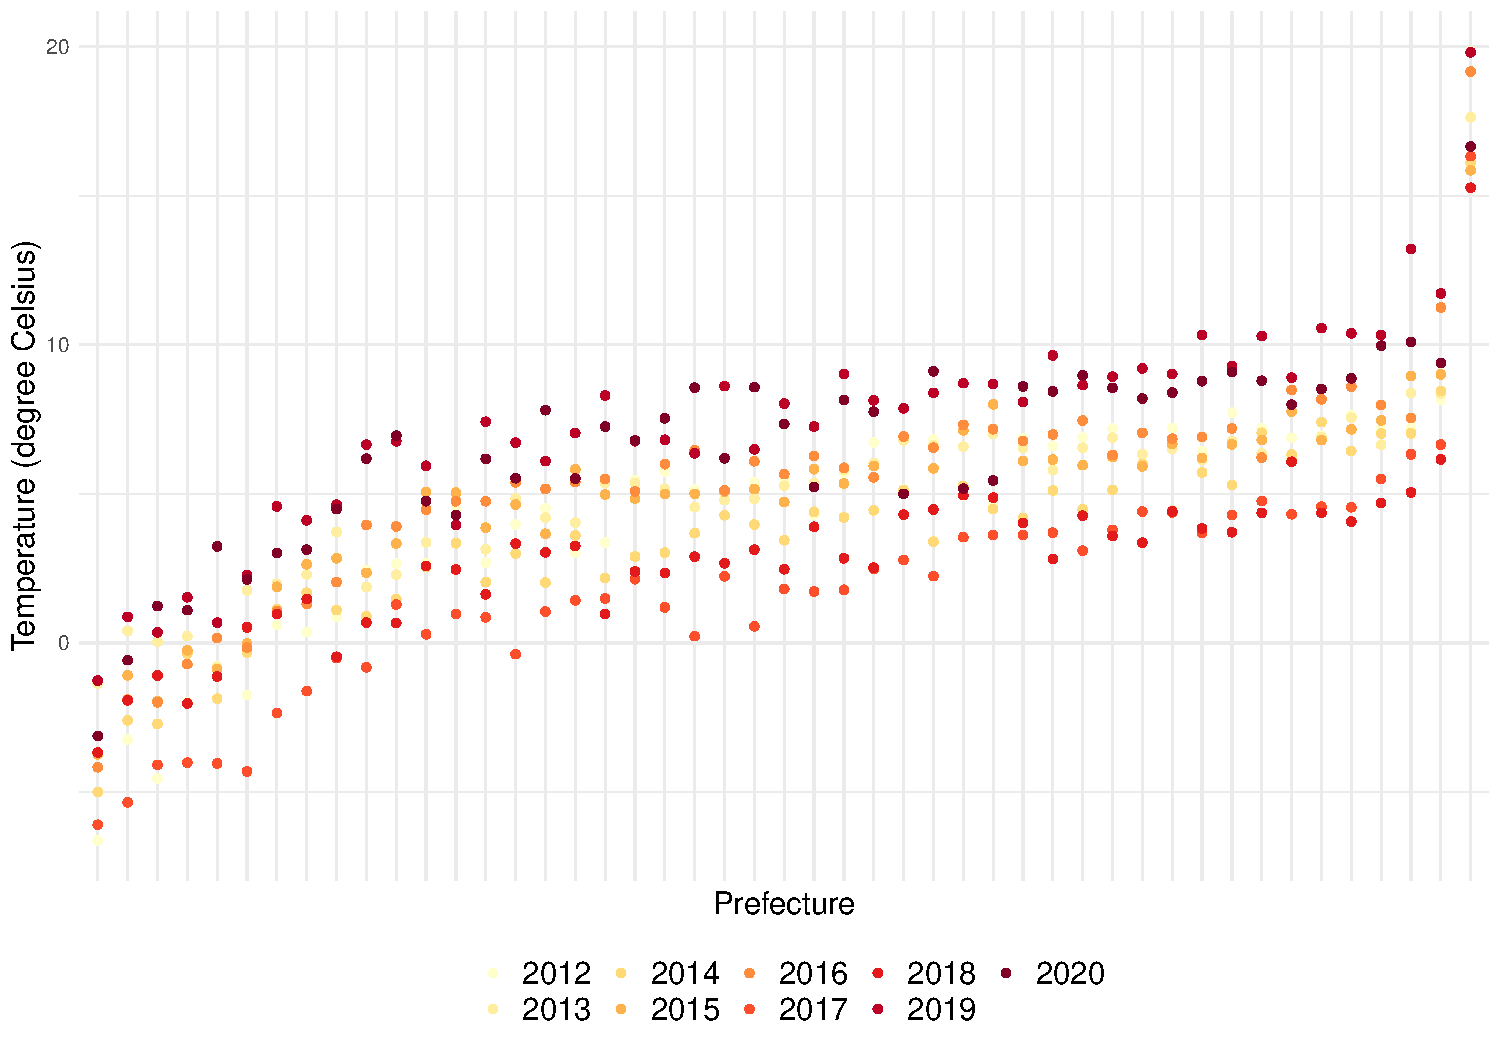
\includegraphics[width = 0.9\textwidth]{../Output/images/temperature_diff.pdf}
  \label{fig:temperature_diff}
  \footnotesize
  \begin{tablenotes}
    \item Notes:
      Temperature at prefecture capitals between 6 AM and 6 PM on days of Center Test is used.
      Average across two test days in each year is shown in the figure.
      The prefectures are ordered by the mean temperature across years (lowest to left and highest to right).
  \end{tablenotes}
\end{figure}

\section{Results}\label{sec:results}

The main empirical results are provided in Table \ref{tab:main_reg}.
The standard errors are clustered at the prefecture level.
Without other weather variables, the estimates in column (1) show a negative and statistically significant impact of cold weather.
Since the mean matriculation share is $2.08$\%, by reducing the temperature from the reference bin (between 3 and 6 $^o$C) to the lowest temperature bin (below 0 $^o$C), the matriculation share decreases by 9\%.
Moreover, due to the stark skewness in the distribution of matriculation shares, the median matriculation share is $0.79$\%.
Therefore, the same temperature change decreases the matriculation share by 22\% of the median value.

In column (2), I add rainfall and snowfall in the regressions.
While temperature coefficients are barely affected, I find that rainfall and snowfall on the exam dates do not impact the matriculation shares.
In column (3), instead of snowfall on the exam dates, I use cumulated snow on the ground and find its negative impact on the outcome. 
To capture the effect of the existence of a certain amount of snow on the ground, column (4) allows a non-linear effect of cumulated snow.
The result shows that snow on the ground cumulated more than 10 cm ($\approx$ 4 inches) decreases the matriculation share by 0.11 percentage points.
These results suggest that not only temperature but also snow on the ground on the exam dates affect exam performance.

Two points are worth noting.
First, Table \ref{tab:linear_reg} shows the results with linear specifications.
While the point estimates for temperature are positive, which means matriculation shares are higher if an exam is held on warmer days, they are statistically insignificant. 
This could due to the plateau effect of temperature above 6 $^o$C in Table \ref{tab:main_reg}.
Although for a quite different temperature range, similar plateau effects are found in \citet{Park2020a}.
Secondly, following the falsification test in \citet{Cho2017}, I check if weather variables one year after the actual Center Test affect the matriculation shares.
The results in Table \ref{tab:reg_placebo_exam} show not only that the weather one year after Center Test has insignificant impacts on matriculation shares but also including the weather variables one year after Center Test barely changes the coefficients on contemporaneous weather variables.
This indicates that the results in \ref{tab:main_reg} capture the effect of transitory shocks on the exam dates.

\begin{table}[H]
  \center
  \caption{Regression: Matriculation share (\%) and weather on exam dates}
  \footnotesize
  
% Table created by stargazer v.5.2.2 by Marek Hlavac, Harvard University. E-mail: hlavac at fas.harvard.edu
% Date and time: Tue, May 04, 2021 - 11:24:34
\begin{tabular}{@{\extracolsep{5pt}}lcccc} 
\\[-1.8ex]\hline 
\hline \\[-1.8ex] 
 & \multicolumn{4}{c}{\textit{Dependent variable:}} \\ 
\cline{2-5} 
\\[-1.8ex] & \multicolumn{4}{c}{Matriculation share (\%)} \\ 
\\[-1.8ex] & (1) & (2) & (3) & (4)\\ 
\hline \\[-1.8ex] 
 Temperature (\degree C) $\le$ 0 & $-$0.18$^{**}$ & $-$0.19$^{**}$ & $-$0.16$^{**}$ & $-$0.15$^{*}$ \\ 
  & (0.08) & (0.08) & (0.08) & (0.08) \\ 
  & & & & \\ 
 Temperature (\degree C) 0-3 & $-$0.08$^{*}$ & $-$0.08$^{*}$ & $-$0.08$^{*}$ & $-$0.08$^{*}$ \\ 
  & (0.04) & (0.04) & (0.04) & (0.04) \\ 
  & & & & \\ 
 Temperature (\degree C) 6-9 & 0.13 & 0.13 & 0.13 & 0.13 \\ 
  & (0.10) & (0.09) & (0.09) & (0.09) \\ 
  & & & & \\ 
 Temperature (\degree C) $>$ 9 & 0.14 & 0.14 & 0.15 & 0.15 \\ 
  & (0.12) & (0.12) & (0.12) & (0.12) \\ 
  & & & & \\ 
 Rainfall (mm) &  & $-$0.02 & 0.06 & 0.06 \\ 
  &  & (0.09) & (0.08) & (0.08) \\ 
  & & & & \\ 
 Snowfall (m) &  & 7.75 &  &  \\ 
  &  & (9.95) &  &  \\ 
  & & & & \\ 
 Cumulated snow (m) &  &  & $-$0.19$^{**}$ &  \\ 
  &  &  & (0.09) &  \\ 
  & & & & \\ 
 Cumulated snow $>$ .10 m &  &  &  & $-$0.11$^{***}$ \\ 
  &  &  &  & (0.04) \\ 
  & & & & \\ 
\hline \\[-1.8ex] 
Prefecture FE & Yes & Yes & Yes & Yes \\ 
Year FE & Yes & Yes & Yes & Yes \\ 
Observations & 423 & 423 & 423 & 423 \\ 
\hline 
\hline \\[-1.8ex] 
\textit{Note:}  & \multicolumn{4}{r}{$^{*}$p$<$0.1; $^{**}$p$<$0.05; $^{***}$p$<$0.01} \\ 
\end{tabular} 

  \label{tab:main_reg}
  \small
  \begin{tablenotes}
    \item
      The outcome variable is the matriculation shares (\%) for the University of Tokyo from each prefecture.
      The matriculation share is calculated based on the ratio of the number of students from high schools in the prefecture to the total number of matriculation.
      I use weather variables at prefecture capitals between 6 AM and 6 PM on days of Center Test.
      Temperature intervals do not contain the right ends.
      Standard errors are clustered at the prefecture level.
  \end{tablenotes}
\end{table}

One possible interpretation of the results is that the estimates in Table \ref{tab:main_reg} reflect the effects of weather on preparation for the exam.
For instance, cold weather can make it hard for students to focus on studying, as suggested by existing studies \citep{Taylor2016}.
Also, snowfall can prevent students from going to high schools or cram schools for studying.
Due to serial correlation between the weather on exam dates and the weather days or weeks before the exam, my regression in Table \ref{tab:main_reg} could capture these effects.
To investigate this possibility, I use the average weather variables for 10 days before the exams and run regressions.
The results in columns (1) and (2) in Table \ref{tab:reg_pre10} show statistically insignificant estimates for the temperature variables.
Moreover, including the weather variables for 10 days before the exams barely changes the estimates on the weather variables on the exam dates (columns (3) and (4)).
These suggest that the negative impacts of low temperature found in Table \ref{tab:main_reg} are mainly caused by the temperature on exam dates rather than temperature before exams.

In columns (1) and (2), the coefficients on snowfall and cumulated snow on the ground are statistically significant.
Combined with the finding in Table \ref{tab:main_reg} that cumulated snow on the ground on the exam dates decreases students' performance, two potential explanations can be given:
(i) snow before the exams can adversely affect students' preparation due to, for instance, more difficulty in going to high schools or cram schools, and
(ii) snowfall before the exams cumulates snow on the ground and students' performance is negatively affected by the cumulated snow on the exam dates.
Including the weather variables on the exam dates, columns (3) and (4) show that only cumulated snow on exam dates has significant impact on the outcome.
This suggests that the second mechanism is dominant.

\begin{table}[H]
  \center
  \caption{Regression: Matriculation share (\%) and average weather for 10 days before exam}
  \scriptsize
  
% Table created by stargazer v.5.2.2 by Marek Hlavac, Harvard University. E-mail: hlavac at fas.harvard.edu
% Date and time: Fri, Apr 02, 2021 - 13:40:23
\begin{tabular}{@{\extracolsep{5pt}}lcccc} 
\\[-1.8ex]\hline 
\hline \\[-1.8ex] 
 & \multicolumn{4}{c}{\textit{Dependent variable:}} \\ 
\cline{2-5} 
\\[-1.8ex] & \multicolumn{4}{c}{Matriculation share (\%)} \\ 
\\[-1.8ex] & (1) & (2) & (3) & (4)\\ 
\hline \\[-1.8ex] 
 Temperature (degree C) & $-$0.01 &  & $-$0.01 &  \\ 
  & (0.02) &  & (0.02) &  \\ 
  & & & & \\ 
 Temperature $\le$ 0 &  & $-$0.03 &  & 0.03 \\ 
  &  & (0.08) &  & (0.09) \\ 
  & & & & \\ 
 Temperature $>$ 0, $\le$ 3 &  & 0.03 &  & 0.05 \\ 
  &  & (0.05) &  & (0.05) \\ 
  & & & & \\ 
 Temperature $>$ 6, $\le$ 9 &  & 0.09 &  & 0.10 \\ 
  &  & (0.06) &  & (0.06) \\ 
  & & & & \\ 
 Temperature $>$ 9 &  & 0.001 &  & 0.02 \\ 
  &  & (0.11) &  & (0.11) \\ 
  & & & & \\ 
 Rainfall (mm) &  &  & $-$0.01 & $-$0.003 \\ 
  &  &  & (0.01) & (0.01) \\ 
  & & & & \\ 
 Snowfall (m) &  &  & $-$0.01 & $-$0.02 \\ 
  &  &  & (0.01) & (0.01) \\ 
  & & & & \\ 
 Cumulated snow (m) &  &  & $-$0.001 & $-$0.001 \\ 
  &  &  & (0.001) & (0.001) \\ 
  & & & & \\ 
\hline \\[-1.8ex] 
Prefecture FE & Yes & Yes & Yes & Yes \\ 
Year FE & Yes & Yes & Yes & Yes \\ 
Observations & 423 & 423 & 423 & 423 \\ 
\hline 
\hline \\[-1.8ex] 
\textit{Note:}  & \multicolumn{4}{r}{$^{*}$p$<$0.1; $^{**}$p$<$0.05; $^{***}$p$<$0.01} \\ 
\end{tabular} 

  \label{tab:reg_pre10}
  \scriptsize
  \begin{tablenotes}
    \item
      The outcome variable is the matriculation shares (\%) for the University of Tokyo from each prefecture.
      The matriculation share is calculated based on the ratio of the number of students from high schools in the prefecture to the total number of matriculation.
      For weather variables with "(exam dates)", I use weather variables at prefecture capitals between 6 AM and 6 PM on days of Center Test.
      For weather variables with "(previous 10 days)", I use their averages at prefecture capitals between 10 days before and 1 day before the first day of Center Test.
      Temperature intervals do not contain the right ends.
      Standard errors are clustered at the prefecture level.
  \end{tablenotes}
\end{table}

\section{Conclusion}\label{sec:conclusion}

This paper studies the impact of winter weather on cognitive performance on a high-stakes exam in Japan.
I use the matriculation share for the most prestigious university in Japan, the University of Tokyo, as an outcome.
Most of the existing studies in the literature have focused on the effect of heat on cognitive performance, while the impact of cold weather remains largely unknown.
This study fills the gap by identifying the causal impact of winter weather on exam results.

The results show both economically and statistically significant impacts of low temperature and cumulated snow on the ground on the exam dates.
Changing the temperature from 3-6 $^o$C to below 0 $^o$C decreases the matriculation share of a prefecture by 0.18 percentage points, which is 9\% of the mean matriculation share, or 22\% of the median matriculation share.
Moreover, having more than 10cm of snow on the ground decreases the share by 0.11 percentage points.

The results in this study have implications for the admissions process of universities.
Recognizing the limitation to measure students' cognitive ability through an exam affected by external factors such as weather, universities may use other measures to select students.
Examples include extracurricular activities and personal statements, which are actively utilized in other countries such as the United States.
Also, universities may adjust the weights for Center Test and the second-stage exam.
Since the second-stage exams are held at each university, all exam takers are exposed to similar environments.
This rules out the possibility that exam takers at different places are affected differently by their conditions.
Given the importance of exam results for later life outcomes of students, it is desirable that universities take measures to mitigate the effect of seemingly irrelevant factors on admission.

\clearpage
\bibliographystyle{apalike}
\bibliography{todai}

%\section{Figures}
%
%\begin{figure}[H]
%  \centering
%  \caption{Map of matriculation shares (\%)}
%  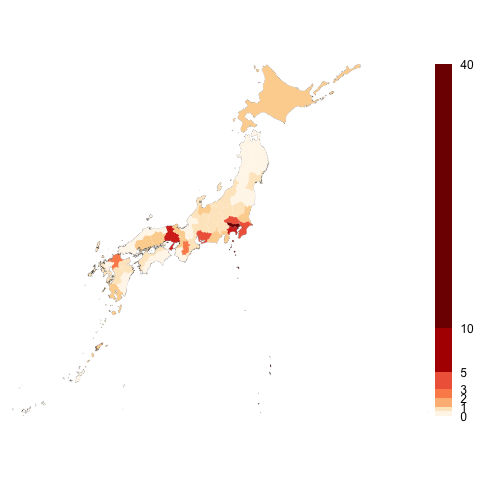
\includegraphics[width = 0.7\textwidth]{../Output/images/admission_map.png}
%  \label{fig:admission_map}
%  \footnotesize
%  \begin{tablenotes}
%    \item Notes:
%      This map shows the matriculation shares (\%) for the University of Tokyo from each prefecture.
%      The matriculation share is calculated based on the ratio of the number of students from high schools in the prefecture to the total number of matriculation.
%      Average of the shares across years is shown in the map.
%      Although not shown in the legend due to the lack of the space, the lightest color in the map means the matriculation share between 0 to 0.5\% 
%  \end{tablenotes}
%\end{figure}
%
%\begin{figure}[H]
%  \centering
%  \caption{Average temperature on two exam dates in each prefecture each year}
%  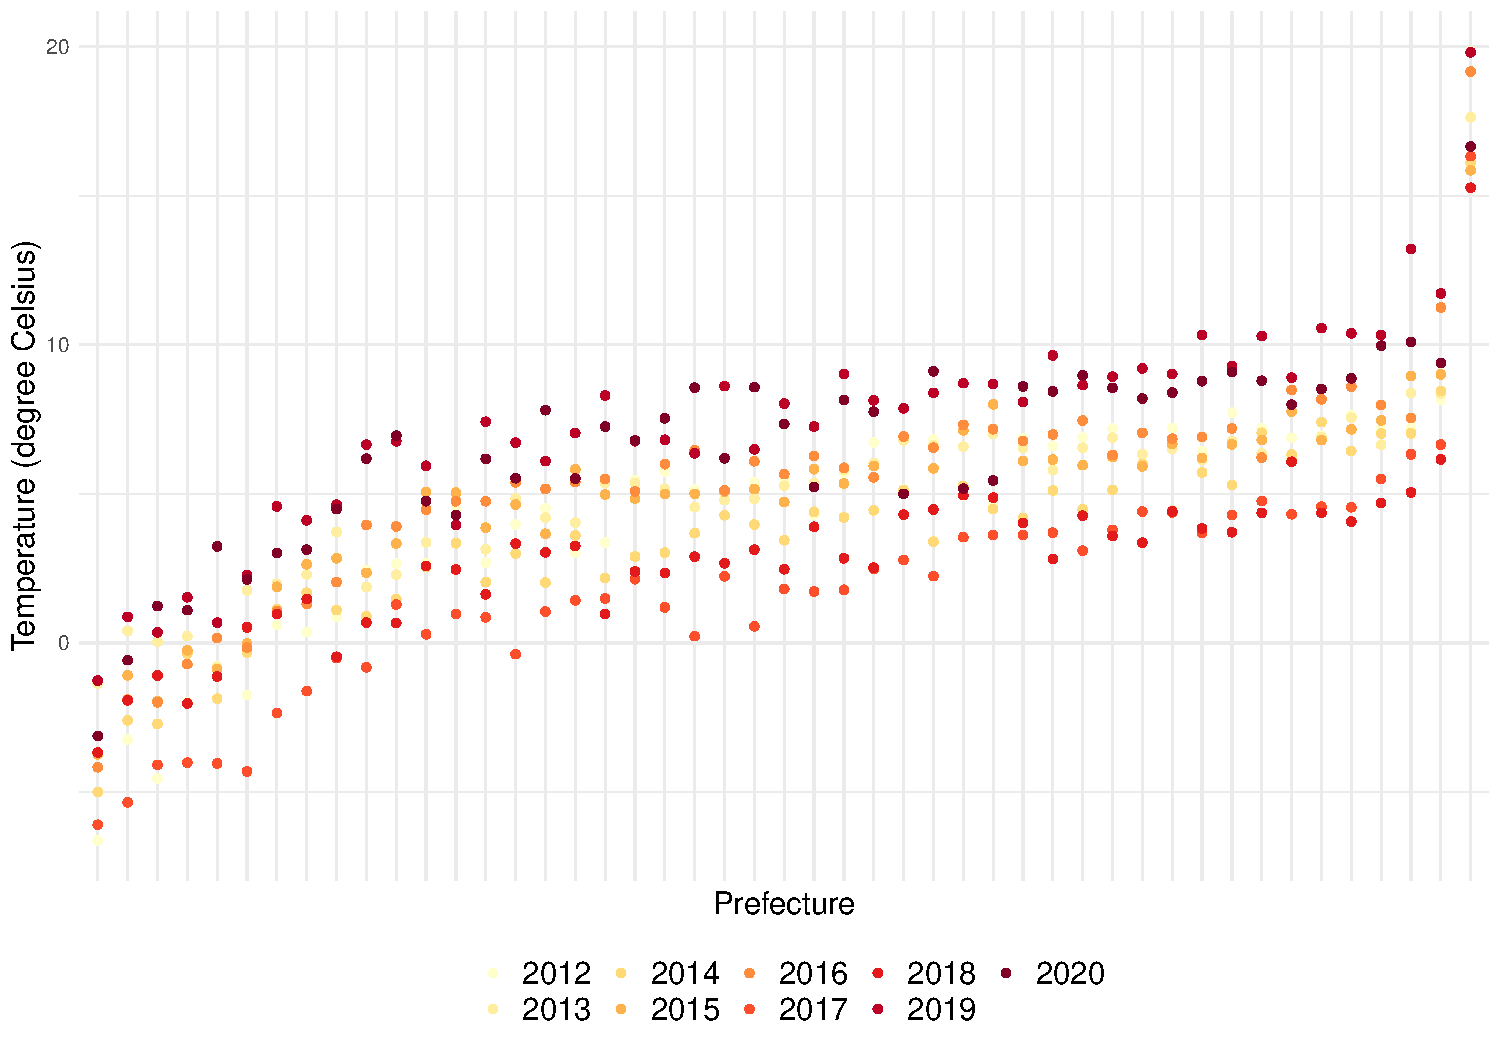
\includegraphics[width = 0.9\textwidth]{../Output/images/temperature_diff.pdf}
%  \label{fig:temperature_diff}
%  \footnotesize
%  \begin{tablenotes}
%    \item Notes:
%      Temperature at prefecture capitals between 6 AM and 6 PM on days of Center Test is used.
%      Average across two test days in each year is shown in the figure.
%      Prefectures positioned to the left on the x-axis are located at more northern parts of Japan.
%  \end{tablenotes}
%\end{figure}
%
%\section{Tables}
%
%\begin{table}[H]
%  \centering
%  \caption{Summary Statistics}
%  \resizebox{0.8\linewidth}{!}{
%  
\begin{tabular}[t]{lllllll}
\toprule
\multicolumn{1}{c}{ } & \multicolumn{1}{c}{N} & \multicolumn{1}{c}{Mean} & \multicolumn{1}{c}{SD} & \multicolumn{1}{c}{Median} & \multicolumn{1}{c}{Min} & \multicolumn{1}{c}{Max} \\
\cmidrule(l{3pt}r{3pt}){2-2} \cmidrule(l{3pt}r{3pt}){3-3} \cmidrule(l{3pt}r{3pt}){4-4} \cmidrule(l{3pt}r{3pt}){5-5} \cmidrule(l{3pt}r{3pt}){6-6} \cmidrule(l{3pt}r{3pt}){7-7}
Matriculation share (\%) & 423 & 2.08 & 5.23 & 0.79 & 0.06 & 37.35\\
Temperature (\degree C) & 423 & 4.67 & 3.81 & 4.98 & -6.63 & 19.86\\
Hourly precipitation (mm) & 423 & 0.08 & 0.18 & 0.00 & 0.00 & 1.27\\
Hourly snowfall (m) & 423 & 0.00 & 0.00 & 0.00 & 0.00 & 0.01\\
Cumulated snow (m) & 423 & 0.05 & 0.15 & 0.00 & 0.00 & 1.26\\
\bottomrule
\end{tabular}

%  }
%  \label{tab:sum_stat}
%  \footnotesize
%  \begin{tablenotes}
%    \item 
%      Notes:
%      Matriculation share (\%) is the share of newly matriculated students to the University of Tokyo from each prefecture.
%      The matriculation share is calculated based on the ratio of the number of students from high schools in the prefecture to the total number of matriculation.
%      I use weather variables at prefecture capitals between 6 AM and 6 PM on days of Center Test.
%  \end{tablenotes}
%\end{table}
%
%\begin{table}[H]
%  \center
%  \caption{Regression: Matriculation share (\%) and weather on exam dates}
%  \small
%  
% Table created by stargazer v.5.2.2 by Marek Hlavac, Harvard University. E-mail: hlavac at fas.harvard.edu
% Date and time: Tue, May 04, 2021 - 11:24:34
\begin{tabular}{@{\extracolsep{5pt}}lcccc} 
\\[-1.8ex]\hline 
\hline \\[-1.8ex] 
 & \multicolumn{4}{c}{\textit{Dependent variable:}} \\ 
\cline{2-5} 
\\[-1.8ex] & \multicolumn{4}{c}{Matriculation share (\%)} \\ 
\\[-1.8ex] & (1) & (2) & (3) & (4)\\ 
\hline \\[-1.8ex] 
 Temperature (\degree C) $\le$ 0 & $-$0.18$^{**}$ & $-$0.19$^{**}$ & $-$0.16$^{**}$ & $-$0.15$^{*}$ \\ 
  & (0.08) & (0.08) & (0.08) & (0.08) \\ 
  & & & & \\ 
 Temperature (\degree C) 0-3 & $-$0.08$^{*}$ & $-$0.08$^{*}$ & $-$0.08$^{*}$ & $-$0.08$^{*}$ \\ 
  & (0.04) & (0.04) & (0.04) & (0.04) \\ 
  & & & & \\ 
 Temperature (\degree C) 6-9 & 0.13 & 0.13 & 0.13 & 0.13 \\ 
  & (0.10) & (0.09) & (0.09) & (0.09) \\ 
  & & & & \\ 
 Temperature (\degree C) $>$ 9 & 0.14 & 0.14 & 0.15 & 0.15 \\ 
  & (0.12) & (0.12) & (0.12) & (0.12) \\ 
  & & & & \\ 
 Rainfall (mm) &  & $-$0.02 & 0.06 & 0.06 \\ 
  &  & (0.09) & (0.08) & (0.08) \\ 
  & & & & \\ 
 Snowfall (m) &  & 7.75 &  &  \\ 
  &  & (9.95) &  &  \\ 
  & & & & \\ 
 Cumulated snow (m) &  &  & $-$0.19$^{**}$ &  \\ 
  &  &  & (0.09) &  \\ 
  & & & & \\ 
 Cumulated snow $>$ .10 m &  &  &  & $-$0.11$^{***}$ \\ 
  &  &  &  & (0.04) \\ 
  & & & & \\ 
\hline \\[-1.8ex] 
Prefecture FE & Yes & Yes & Yes & Yes \\ 
Year FE & Yes & Yes & Yes & Yes \\ 
Observations & 423 & 423 & 423 & 423 \\ 
\hline 
\hline \\[-1.8ex] 
\textit{Note:}  & \multicolumn{4}{r}{$^{*}$p$<$0.1; $^{**}$p$<$0.05; $^{***}$p$<$0.01} \\ 
\end{tabular} 

%  \label{tab:main_reg}
%  \small
%  \begin{tablenotes}
%    \item
%      The outcome variable is the matriculation shares (\%) for the University of Tokyo from each prefecture.
%      The matriculation share is calculated based on the ratio of the number of students from high schools in the prefecture to the total number of matriculation.
%      I use weather variables at prefecture capitals between 6 AM and 6 PM on days of Center Test.
%      Standard errors are clustered at the prefecture level.
%  \end{tablenotes}
%\end{table}
%
%\begin{table}[H]
%  \center
%  \caption{Regression: Matriculation share (\%) and average weather for 10 days before exam}
%  
% Table created by stargazer v.5.2.2 by Marek Hlavac, Harvard University. E-mail: hlavac at fas.harvard.edu
% Date and time: Fri, Apr 02, 2021 - 13:40:23
\begin{tabular}{@{\extracolsep{5pt}}lcccc} 
\\[-1.8ex]\hline 
\hline \\[-1.8ex] 
 & \multicolumn{4}{c}{\textit{Dependent variable:}} \\ 
\cline{2-5} 
\\[-1.8ex] & \multicolumn{4}{c}{Matriculation share (\%)} \\ 
\\[-1.8ex] & (1) & (2) & (3) & (4)\\ 
\hline \\[-1.8ex] 
 Temperature (degree C) & $-$0.01 &  & $-$0.01 &  \\ 
  & (0.02) &  & (0.02) &  \\ 
  & & & & \\ 
 Temperature $\le$ 0 &  & $-$0.03 &  & 0.03 \\ 
  &  & (0.08) &  & (0.09) \\ 
  & & & & \\ 
 Temperature $>$ 0, $\le$ 3 &  & 0.03 &  & 0.05 \\ 
  &  & (0.05) &  & (0.05) \\ 
  & & & & \\ 
 Temperature $>$ 6, $\le$ 9 &  & 0.09 &  & 0.10 \\ 
  &  & (0.06) &  & (0.06) \\ 
  & & & & \\ 
 Temperature $>$ 9 &  & 0.001 &  & 0.02 \\ 
  &  & (0.11) &  & (0.11) \\ 
  & & & & \\ 
 Rainfall (mm) &  &  & $-$0.01 & $-$0.003 \\ 
  &  &  & (0.01) & (0.01) \\ 
  & & & & \\ 
 Snowfall (m) &  &  & $-$0.01 & $-$0.02 \\ 
  &  &  & (0.01) & (0.01) \\ 
  & & & & \\ 
 Cumulated snow (m) &  &  & $-$0.001 & $-$0.001 \\ 
  &  &  & (0.001) & (0.001) \\ 
  & & & & \\ 
\hline \\[-1.8ex] 
Prefecture FE & Yes & Yes & Yes & Yes \\ 
Year FE & Yes & Yes & Yes & Yes \\ 
Observations & 423 & 423 & 423 & 423 \\ 
\hline 
\hline \\[-1.8ex] 
\textit{Note:}  & \multicolumn{4}{r}{$^{*}$p$<$0.1; $^{**}$p$<$0.05; $^{***}$p$<$0.01} \\ 
\end{tabular} 

%  \label{tab:reg_pre10}
%  \small
%  \begin{tablenotes}
%    \item
%      The outcome variable is the matriculation shares (\%) for the University of Tokyo from each prefecture.
%      The matriculation share is calculated based on the ratio of the number of students from high schools in the prefecture to the total number of matriculation.
%      I use average weather variables at prefecture capitals between 10 days before and 1 day before the first day of Center Test.
%      Standard errors are clustered at the prefecture level.
%  \end{tablenotes}
%\end{table}

\appendix

\setcounter{figure}{0}
\setcounter{table}{0}
\renewcommand\thefigure{\Alph{section}.\arabic{figure}}
\renewcommand\thetable{\Alph{section}.\arabic{table}}
  
\section{Appendix tables}\label{sec:appendix_table}

%\begin{table}[H]
%  \center
%  \caption{Regression: Matriculation share (\%) and weather on exam dates by gender}
%  
% Table created by stargazer v.5.2.2 by Marek Hlavac, Harvard University. E-mail: hlavac at fas.harvard.edu
% Date and time: Thu, Apr 22, 2021 - 22:43:59
\begin{tabular}{@{\extracolsep{5pt}}lcccc} 
\\[-1.8ex]\hline 
\hline \\[-1.8ex] 
 & \multicolumn{4}{c}{\textit{Dependent variable:}} \\ 
\cline{2-5} 
\\[-1.8ex] & \multicolumn{2}{c}{Matriculation share (\%, female)} & \multicolumn{2}{c}{Matriculation share (\%, male)} \\ 
\\[-1.8ex] & (1) & (2) & (3) & (4)\\ 
\hline \\[-1.8ex] 
 Temperature (\degree C) $\le$ 0 & $-$0.01 & $-$0.01 & $-$0.18$^{**}$ & $-$0.15$^{**}$ \\ 
  & (0.03) & (0.03) & (0.08) & (0.07) \\ 
  & & & & \\ 
 Temperature (\degree C) $>$ 0, $\le$ 3 & 0.02 & 0.02 & $-$0.10$^{*}$ & $-$0.10$^{*}$ \\ 
  & (0.03) & (0.02) & (0.05) & (0.05) \\ 
  & & & & \\ 
 Temperature (\degree C) $>$ 6, $\le$ 9 & 0.04 & 0.04 & 0.09 & 0.10 \\ 
  & (0.03) & (0.03) & (0.07) & (0.07) \\ 
  & & & & \\ 
 Temperature (\degree C) $>$ 9 & 0.06 & 0.06 & 0.07 & 0.09 \\ 
  & (0.04) & (0.04) & (0.09) & (0.09) \\ 
  & & & & \\ 
 Rainfall (mm) & 0.02 & 0.001 & $-$0.04 & 0.06 \\ 
  & (0.05) & (0.03) & (0.12) & (0.08) \\ 
  & & & & \\ 
 Snowfall (m) & $-$7.63 &  & 15.37 &  \\ 
  & (8.38) &  & (14.37) &  \\ 
  & & & & \\ 
 Cumulated snow (m) &  & $-$0.07 &  & $-$0.12 \\ 
  &  & (0.05) &  & (0.08) \\ 
  & & & & \\ 
\hline \\[-1.8ex] 
Prefecture FE & Yes & Yes & Yes & Yes \\ 
Year FE & Yes & Yes & Yes & Yes \\ 
Observations & 423 & 423 & 423 & 423 \\ 
\hline 
\hline \\[-1.8ex] 
\textit{Note:}  & \multicolumn{4}{r}{$^{*}$p$<$0.1; $^{**}$p$<$0.05; $^{***}$p$<$0.01} \\ 
\end{tabular} 

%  \label{tab:reg_by_gender}
%  \small
%  \begin{tablenotes}
%    \item
%      The outcome variable is the matriculation shares (\%) for the University of Tokyo from each prefecture.
%      The matriculation share is calculated based on the ratio of the number of students from high schools in the prefecture to the total number of matriculation.
%      I use weather variables at prefecture capitals between 6 AM and 6 PM on days of Center Test.
%      Standard errors are clustered at the prefecture level.
%  \end{tablenotes}
%\end{table}

\begin{table}[H]
  \center
  \caption{Regression: Matriculation share (\%) and weather on exam dates (linear specification)}
  \small
  
% Table created by stargazer v.5.2.2 by Marek Hlavac, Harvard University. E-mail: hlavac at fas.harvard.edu
% Date and time: Thu, May 13, 2021 - 14:05:22
\begin{tabular}{@{\extracolsep{5pt}}lcccc} 
\\[-1.8ex]\hline 
\hline \\[-1.8ex] 
 & \multicolumn{4}{c}{\textit{Dependent variable:}} \\ 
\cline{2-5} 
\\[-1.8ex] & \multicolumn{4}{c}{Matriculation share (\%)} \\ 
\\[-1.8ex] & (1) & (2) & (3) & (4)\\ 
\hline \\[-1.8ex] 
 Temperature (\degree C) & 0.02 & 0.02 & 0.02 & 0.02 \\ 
  & (0.02) & (0.02) & (0.02) & (0.02) \\ 
  & & & & \\ 
 Rainfall (mm) &  & $-$0.04 & 0.04 & 0.05 \\ 
  &  & (0.10) & (0.08) & (0.09) \\ 
  & & & & \\ 
 Snowfall (cm) &  & 0.08 &  &  \\ 
  &  & (0.11) &  &  \\ 
  & & & & \\ 
 Cumulated snow (cm) &  &  & $-$0.002$^{**}$ &  \\ 
  &  &  & (0.001) &  \\ 
  & & & & \\ 
 Cumulated snow $>$ 10 cm &  &  &  & $-$0.11$^{**}$ \\ 
  &  &  &  & (0.04) \\ 
  & & & & \\ 
\hline \\[-1.8ex] 
Prefecture FE & Yes & Yes & Yes & Yes \\ 
Year FE & Yes & Yes & Yes & Yes \\ 
Observations & 423 & 423 & 423 & 423 \\ 
\hline 
\hline \\[-1.8ex] 
\textit{Note:}  & \multicolumn{4}{r}{$^{*}$p$<$0.1; $^{**}$p$<$0.05; $^{***}$p$<$0.01} \\ 
\end{tabular} 

  \label{tab:linear_reg}
  \small
  \begin{tablenotes}
    \item
      The outcome variable is the matriculation shares (\%) for the University of Tokyo from each prefecture.
      The matriculation share is calculated based on the ratio of the number of students from high schools in the prefecture to the total number of matriculation.
      I use weather variables at prefecture capitals between 6 AM and 6 PM on days of Center Test.
      Standard errors are clustered at the prefecture level.
  \end{tablenotes}
\end{table}

\begin{table}[H]
  \center
  \caption{Falsification test: Matriculation share (\%) and weather on exam dates and one year after}
  \scriptsize
  
% Table created by stargazer v.5.2.2 by Marek Hlavac, Harvard University. E-mail: hlavac at fas.harvard.edu
% Date and time: Thu, Apr 22, 2021 - 22:37:51
\begin{tabular}{@{\extracolsep{5pt}}lcccc} 
\\[-1.8ex]\hline 
\hline \\[-1.8ex] 
 & \multicolumn{4}{c}{\textit{Dependent variable:}} \\ 
\cline{2-5} 
\\[-1.8ex] & \multicolumn{4}{c}{Matriculation share (\%)} \\ 
\\[-1.8ex] & (1) & (2) & (3) & (4)\\ 
\hline \\[-1.8ex] 
 Temperature (\degree C) $\le$ 0 ($t$) &  &  & $-$0.17$^{**}$ & $-$0.14$^{*}$ \\ 
  &  &  & (0.08) & (0.08) \\ 
  & & & & \\ 
 Temperature (\degree C) $>$ 0, $\le$ 3 ($t$) &  &  & $-$0.07$^{*}$ & $-$0.07 \\ 
  &  &  & (0.04) & (0.04) \\ 
  & & & & \\ 
 Temperature (\degree C) $>$ 6, $\le$ 9 ($t$) &  &  & 0.12 & 0.13 \\ 
  &  &  & (0.09) & (0.09) \\ 
  & & & & \\ 
 Temperature (\degree C) $>$ 9 ($t$) &  &  & 0.14 & 0.15 \\ 
  &  &  & (0.11) & (0.11) \\ 
  & & & & \\ 
 Rainfall (mm) ($t$) &  &  & $-$0.07 & 0.04 \\ 
  &  &  & (0.09) & (0.08) \\ 
  & & & & \\ 
 Snowfall (m) ($t$) &  &  & 11.31 &  \\ 
  &  &  & (9.22) &  \\ 
  & & & & \\ 
 Cumulated snow (m) ($t$) &  &  &  & $-$0.22$^{**}$ \\ 
  &  &  &  & (0.09) \\ 
  & & & & \\ 
 Temperature (\degree C) $\le$ 0 ($t + 1$) & 0.02 & $-$0.05 & $-$0.01 & $-$0.03 \\ 
  & (0.12) & (0.11) & (0.11) & (0.10) \\ 
  & & & & \\ 
 Temperature (\degree C) $>$ 0, $\le$ 3 ($t + 1$) & $-$0.03 & $-$0.05 & $-$0.04 & $-$0.05 \\ 
  & (0.05) & (0.05) & (0.05) & (0.05) \\ 
  & & & & \\ 
 Temperature (\degree C) $>$ 6, $\le$ 9 ($t + 1$) & 0.04 & 0.04 & 0.05 & 0.04 \\ 
  & (0.05) & (0.05) & (0.05) & (0.05) \\ 
  & & & & \\ 
 Temperature (\degree C) $>$ 9 ($t + 1$) & $-$0.09 & $-$0.09 & $-$0.05 & $-$0.06 \\ 
  & (0.08) & (0.08) & (0.07) & (0.07) \\ 
  & & & & \\ 
 Rainfall (mm) ($t + 1$) & $-$0.01 & $-$0.03 & $-$0.01 & $-$0.03 \\ 
  & (0.05) & (0.05) & (0.05) & (0.05) \\ 
  & & & & \\ 
 Snowfall (m) ($t + 1$) & $-$9.10 &  & $-$4.94 &  \\ 
  & (12.08) &  & (11.90) &  \\ 
  & & & & \\ 
 Cumulated snow (m) ($t + 1$) &  & 0.13 &  & 0.11 \\ 
  &  & (0.12) &  & (0.12) \\ 
  & & & & \\ 
\hline \\[-1.8ex] 
Prefecture FE & Yes & Yes & Yes & Yes \\ 
Year FE & Yes & Yes & Yes & Yes \\ 
Observations & 423 & 423 & 423 & 423 \\ 
\hline 
\hline \\[-1.8ex] 
\textit{Note:}  & \multicolumn{4}{r}{$^{*}$p$<$0.1; $^{**}$p$<$0.05; $^{***}$p$<$0.01} \\ 
\end{tabular} 

  \label{tab:reg_placebo_exam}
  \scriptsize
  \begin{tablenotes}
    \item
      The outcome variable is the matriculation shares (\%) for the University of Tokyo from each prefecture.
      The matriculation share is calculated based on the ratio of the number of students from high schools in the prefecture to the total number of matriculation.
      I use weather variables at prefecture capitals between 6 AM and 6 PM on days of Center Test.
      I represent the contemporaneous weather variables with ``($t$)'' and the weather one year after Center Test with ``($t + 1$).''
      Temperature intervals do not contain the right ends.
      Standard errors are clustered at the prefecture level.
  \end{tablenotes}
\end{table}

\setcounter{figure}{0}
\setcounter{table}{0}
\renewcommand\thefigure{\Alph{section}.\arabic{figure}}
\renewcommand\thetable{\Alph{section}.\arabic{table}}
  
\section{Appendix figures}\label{sec:appendix_figure}

\begin{figure}[H]
  \centering
  \caption{Average hourly rainfall (m) on two exam dates in each prefecture each year}
  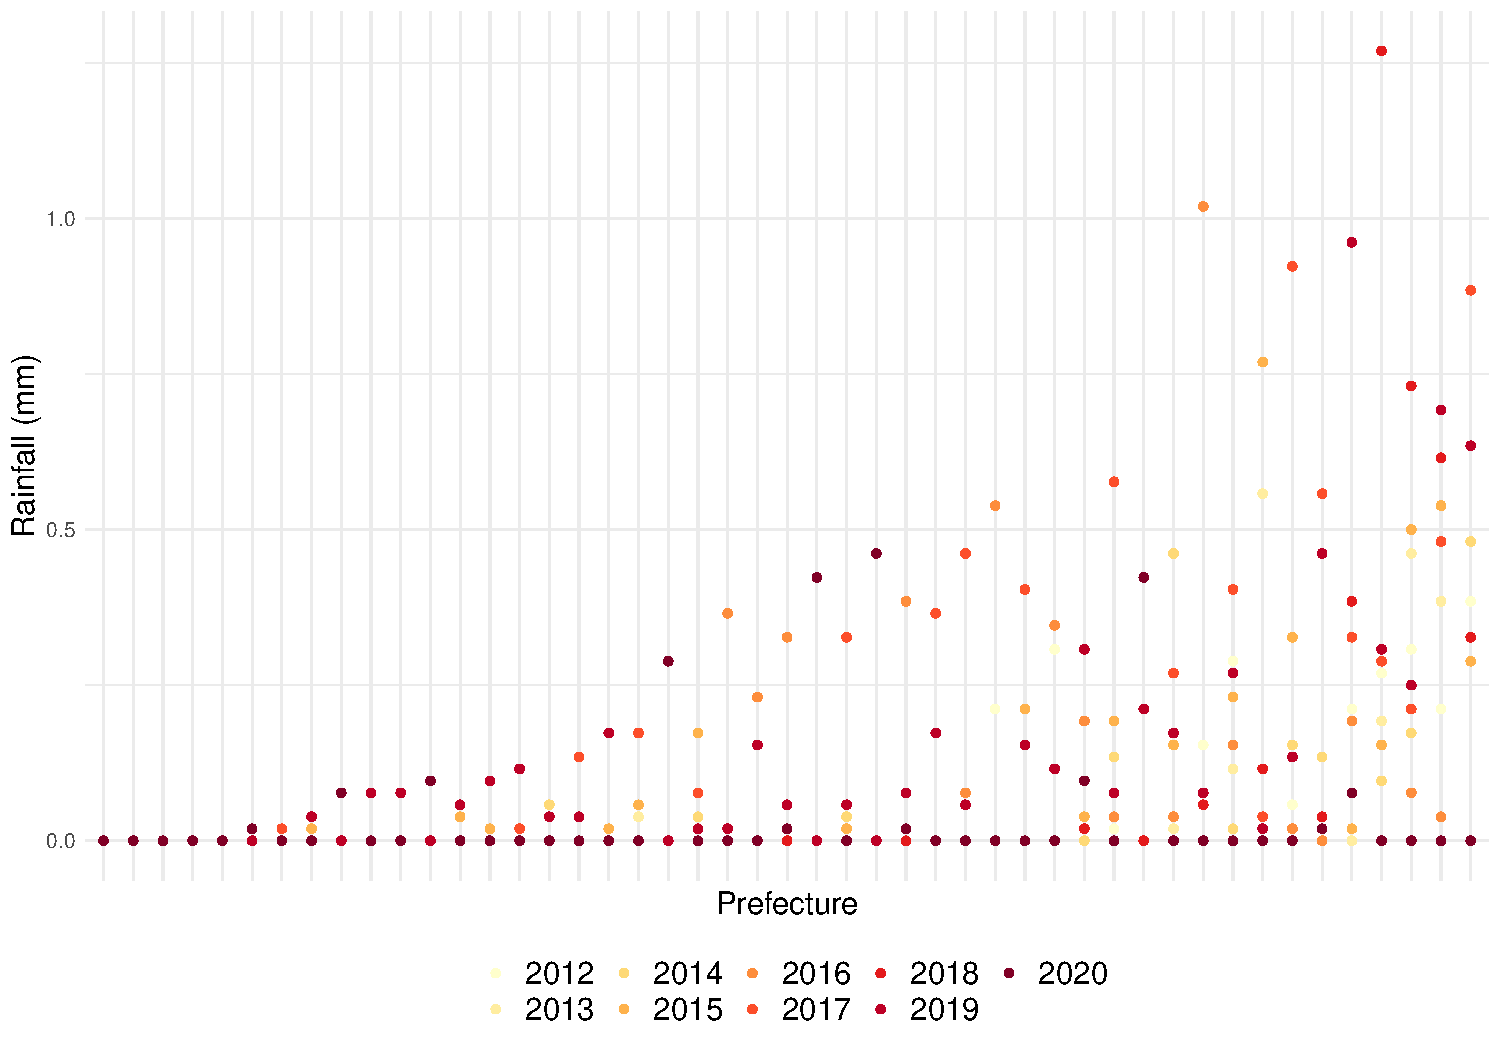
\includegraphics[width = 0.9\textwidth]{../Output/images/rainfall_diff.pdf}
  \label{fig:rainfall_diff}
  \footnotesize
  \begin{tablenotes}
    \item Notes:
      Rainfall (mm) at prefecture capitals between 6 AM and 6 PM on days of Center Test is used.
      Average across two test days in each year is shown in the figure.
      The prefectures are ordered by the mean rainfall across years (lowest to left and highest to right).
  \end{tablenotes}
\end{figure}

\begin{figure}[H]
  \centering
  \caption{Average hourly snowfall (m) on two exam dates in each prefecture each year}
  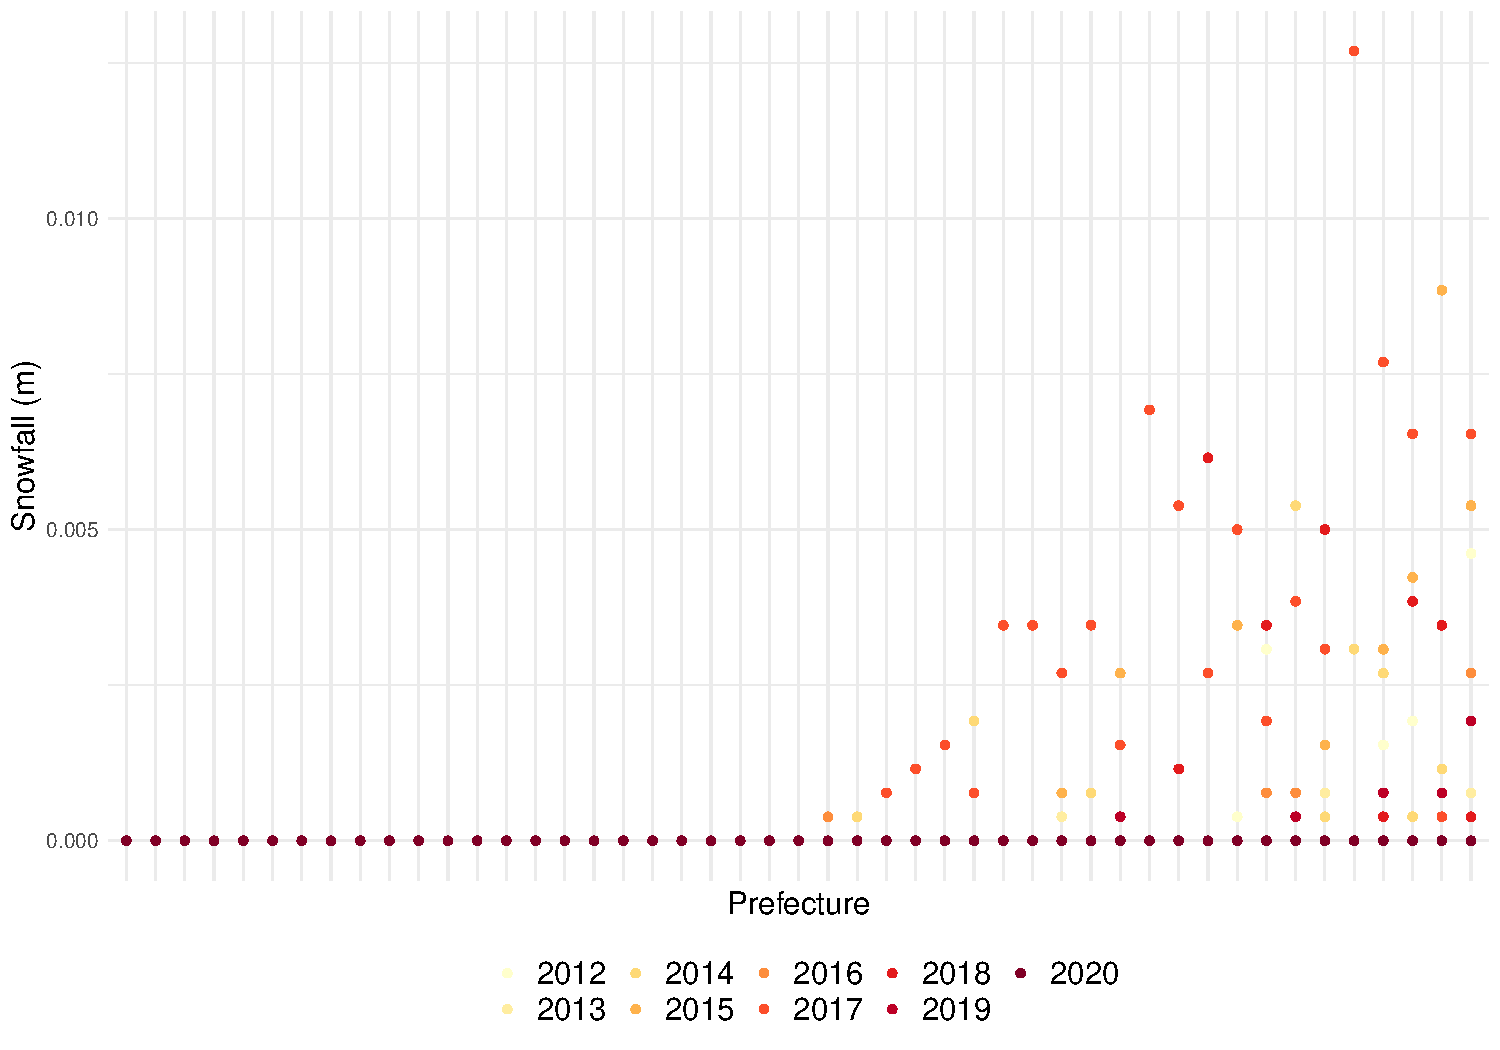
\includegraphics[width = 0.9\textwidth]{../Output/images/snowfall_diff.pdf}
  \label{fig:snowfall_diff}
  \footnotesize
  \begin{tablenotes}
    \item Notes:
      Snowfall (m) at prefecture capitals between 6 AM and 6 PM on days of Center Test is used.
      Average across two test days in each year is shown in the figure.
      The prefectures are ordered by the mean snowfall across years (lowest to left and highest to right).
  \end{tablenotes}
\end{figure}

\begin{figure}[H]
  \centering
  \caption{Average cumulated snow (m) on two exam dates in each prefecture each year}
  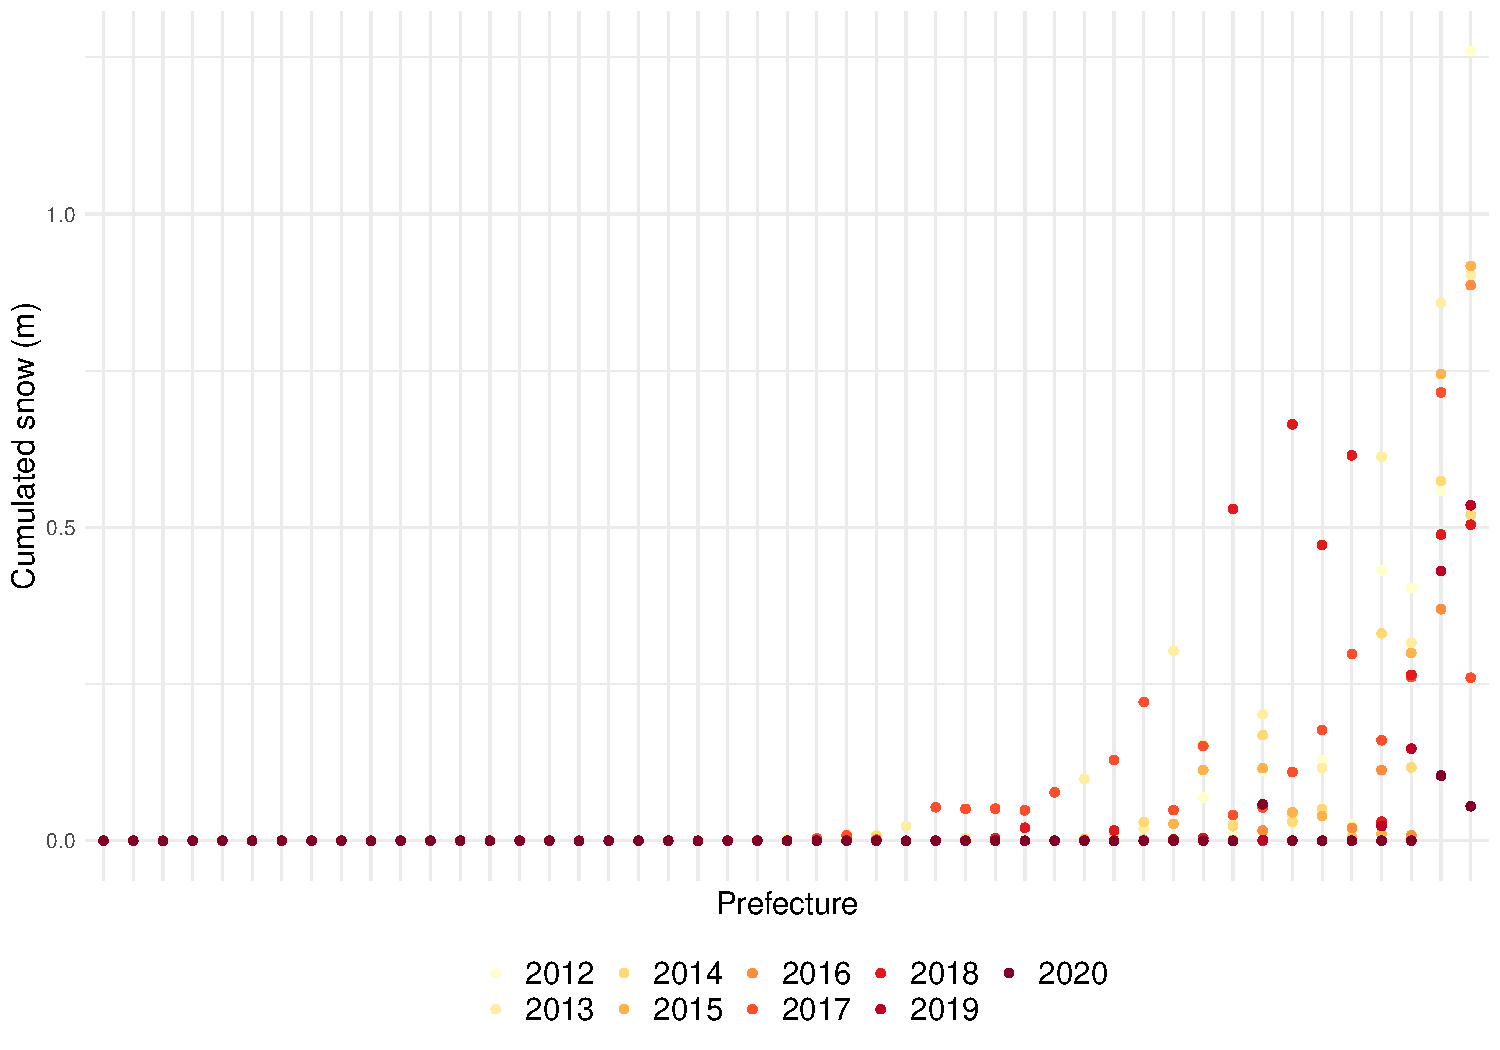
\includegraphics[width = 0.9\textwidth]{../Output/images/cum_snow_diff.pdf}
  \label{fig:cum_snow_diff}
  \footnotesize
  \begin{tablenotes}
    \item Notes:
      Cumulated snow (m) at prefecture capitals between 6 AM and 6 PM on days of Center Test is used.
      Average across two test days in each year is shown in the figure.
      The prefectures are ordered by the mean cumulated snow across years (lowest to left and highest to right).
  \end{tablenotes}
\end{figure}

\begin{figure}[H]
  \centering
  \caption{Deviation of temperatures from within-prefecture averages}
  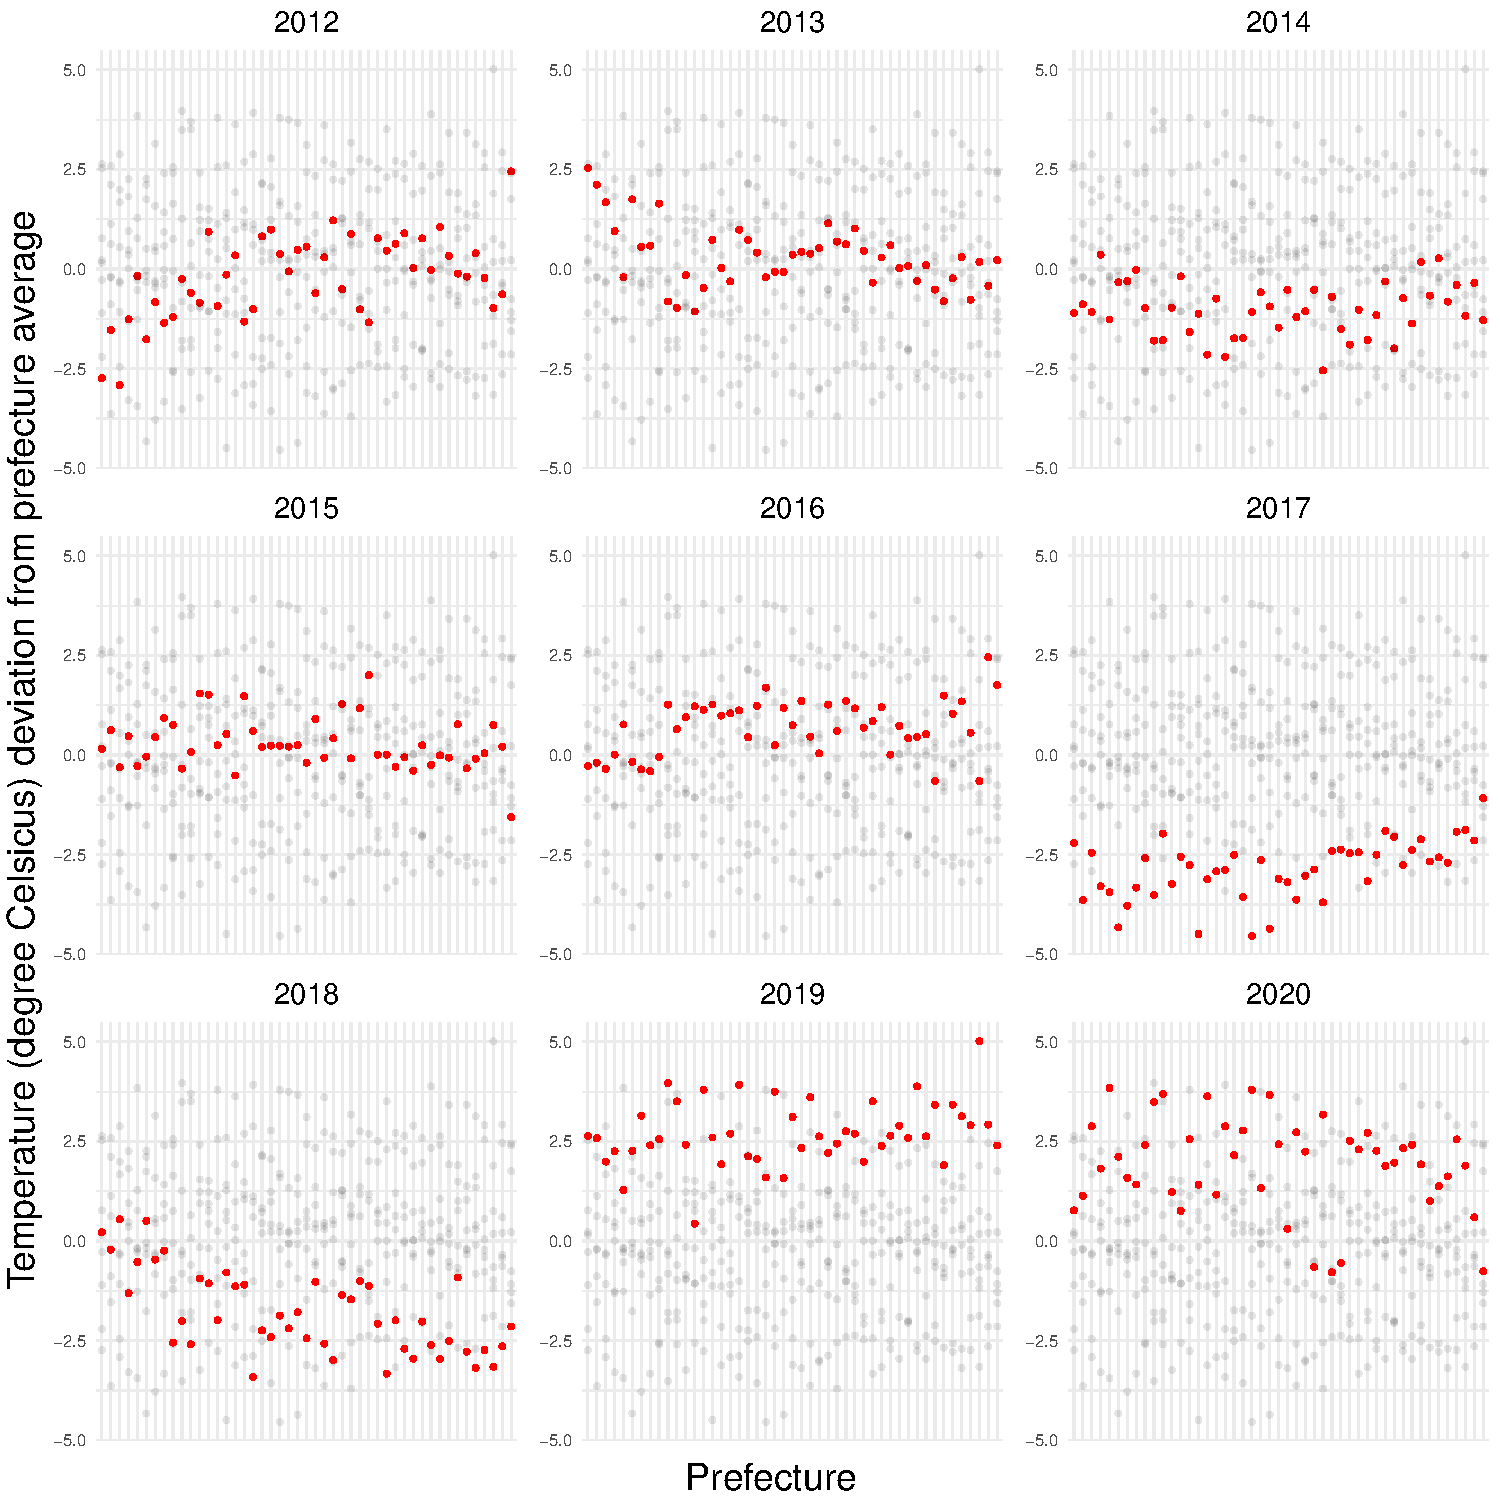
\includegraphics[width = 0.9\textwidth]{../Output/images/temperature_diff_by_year.pdf}
  \label{fig:temperature_diff_by_year}
  \footnotesize
  \begin{tablenotes}
    \item Notes:
      Temperature at prefecture capitals between 6 AM and 6 PM on days of Center Test is used.
      Deviations of average temperatures across two test days from their within-prefecture means are shown in the figure by year.
      In each panel, red dots are the deviations in the year shown above and gray dots are the deviations in the other years.
      The prefectures are ordered by the mean temperature across years (lowest to left and highest to right).
  \end{tablenotes}
\end{figure}

%\begin{figure}[H]
%  \centering
%  \caption{Map of average temperature on two exam dates (average across years)}
%  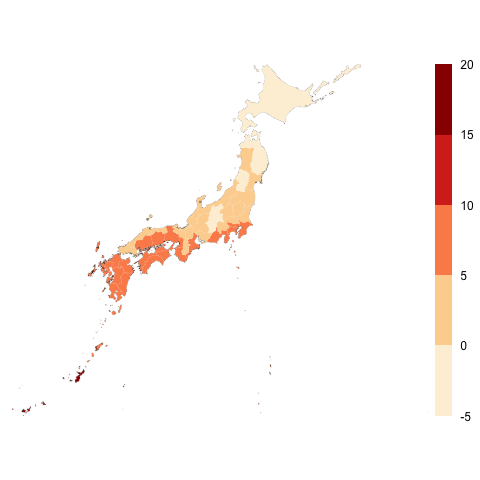
\includegraphics[width = 0.9\textwidth]{../Output/images/temperature_map.png}
%  \label{fig:temperature_map}
%  \footnotesize
%  \begin{tablenotes}
%    \item Notes:
%      Temperature at prefecture capitals between 6 AM and 6 PM on days of Center Test is used.
%      Average of the temperatures across years is shown in the map.
%  \end{tablenotes}
%\end{figure}
%
%\begin{figure}[H]
%  \centering
%  \caption{Map of average cumulated snow (m) on two exam dates (average across years)}
%  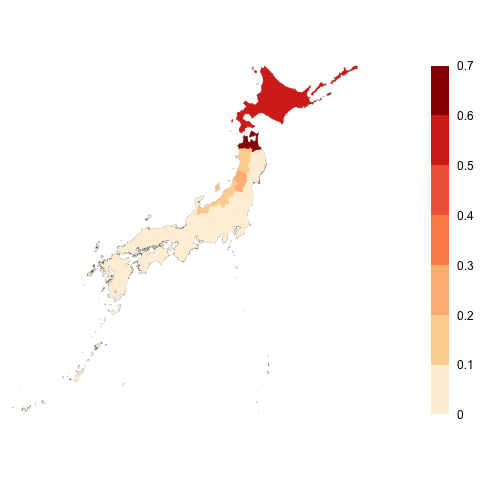
\includegraphics[width = 0.9\textwidth]{../Output/images/cum_snow_map.png}
%  \label{fig:cum_snow_map}
%  \footnotesize
%  \begin{tablenotes}
%    \item Notes:
%      Cumulated snow (m) on the ground at prefecture capitals between 6 AM and 6 PM on days of Center Test is used.
%      Average of the values across years is shown in the map.
%  \end{tablenotes}
%\end{figure}

  
\end{document}



